% !TeX document-id = {acae32e8-6141-4de2-ac12-2af5cc72aa20}
% !TeX encoding = utf8
% !TeX spellcheck = br_PT
% !TeX program = pdflatex
% !BIB program = bibtex
%%
%% This is file `example.tex',
%% generated with the docstrip utility.
%%
%% The original source files were:
%%
%% coppe.dtx  (with options: `example')
%%
%% This is a sample monograph which illustrates the use of `coppe' document
%% class and `coppe-unsrt' BibTeX style.
%%
%% \CheckSum{1613}
%% \CharacterTable
%%  {Upper-case    \A\B\C\D\E\F\G\H\I\J\K\L\M\N\O\P\Q\R\S\T\U\V\W\X\Y\Z
%%   Lower-case    \a\b\c\d\e\f\g\h\i\j\k\l\m\n\o\p\q\r\s\t\u\v\w\x\y\z
%%   Digits        \0\1\2\3\4\5\6\7\8\9
%%   Exclamation   \!     Double quote  \"     Hash (number) \#
%%   Dollar        \$     Percent       \%     Ampersand     \&
%%   Acute accent  \'     Left paren    \(     Right paren   \)
%%   Asterisk      \*     Plus          \+     Comma         \,
%%   Minus         \-     Point         \.     Solidus       \/
%%   Colon         \:     Semicolon     \;     Less than     \<
%%   Equals        \=     Greater than  \>     Question mark \?
%%   Commercial at \@     Left bracket  \[     Backslash     \\
%%   Right bracket \]     Circumflex    \^     Underscore    \_
%%   Grave accent  \`     Left brace    \{     Vertical bar  \|
%%   Right brace   \}     Tilde         \~}
%%
\documentclass[dsc,numbers]{coppe}
\usepackage{amsmath,amssymb}
\usepackage[editing]{../../coop-writing}
\usepackage{hyperref}


\makelosymbols
\makeloabbreviations

\begin{document}
  \title{T\'itulo da Tese}
  \foreigntitle{Thesis Title}
  \author{Nome do Autor}{Sobrenome}
  \advisor{Prof.}{Nome do Primeiro Orientador}{Sobrenome}{D.Sc.}
  \advisor{Prof.}{Nome do Segundo Orientador}{Sobrenome}{Ph.D.}
  \advisor{Prof.}{Nome do Terceiro Orientador}{Sobrenome}{D.Sc.}

  \examiner{Prof.}{Nome do Primeiro Examinador Sobrenome}{D.Sc.}
  \examiner{Prof.}{Nome do Segundo Examinador Sobrenome}{Ph.D.}
  \examiner{Prof.}{Nome do Terceiro Examinador Sobrenome}{D.Sc.}
  \examiner{Prof.}{Nome do Quarto Examinador Sobrenome}{Ph.D.}
  \examiner{Prof.}{Nome do Quinto Examinador Sobrenome}{Ph.D.}
  \department{PEC}
  \date{02}{2011}

  \keyword{Primeira palavra-chave}
  \keyword{Segunda palavra-chave}
  \keyword{Terceira palavra-chave}

  \maketitle

  \frontmatter
  \dedication{A algu\'em cujo valor \'e digno desta dedicat\'oria.}

  \chapter*{Agradecimentos}

  Gostaria de agradecer a todos.

  \begin{abstract}

  Apresenta-se, nesta tese, ...

  \end{abstract}

  \begin{foreignabstract}

  In this work, we present ...

  \end{foreignabstract}

  \tableofcontents
  \listoffigures
  \listoftables
  \printlosymbols
  \printloabbreviations

  \mainmatter
  \chapter{Introdu{\c c}\~ao}

  Segundo a norma de formata{\c c}\~ao de teses e disserta{\c c}\~oes do
  Instituto Alberto Luiz Coimbra de P\'os-gradua{\c c}\~ao e Pesquisa de
  Engenharia (COPPE), toda abreviatura deve ser definida antes de
  utilizada.\abbrev{COPPE}{Instituto Alberto Luiz Coimbra de P\'os-gradua{\c
  c}\~ao e Pesquisa de Engenharia}

  Do mesmo modo, \'e imprescind\'ivel definir os s\'imbolos, tal como o
  conjunto dos n\'umeros reais $\mathbb{R}$ e o conjunto vazio $\emptyset$.
  \symbl{$\mathbb{R}$}{Conjunto dos n\'umeros reais}
  \symbl{$\emptyset$}{Conjunto vazio}

  \begin{longquote}
  Um exemplo de citação longa nas regras da ABNT (4cm de recuo e fonte menor)
  feita com o ambiente  \verb=longquote= The primary objective of this
  investigation was to determine the feasibility of detecting corrosion in
  aluminum Naval aircraft components with neutron radiographic interrogation
  and the use of standard corrosion penetrameters. Secondary objectives
  included the determination of the effect of object thickness on image quality,
  the defining of minimum levels of detectability and a preliminary investigation
  of a means whereby the degree of corrosion could be quantified with neutron
  radiographic data. \cite{article-example}
  \end{longquote}

  \chapter{Revis\~ao Bibliogr\'afica}

  Para ilustrar a completa ades\~ao ao estilo de cita{\c c}\~oes e listagem de
  refer\^encias bibliogr\'aficas, a Tabela~\ref{tab:citation} apresenta cita{\c
  c}\~oes de alguns dos trabalhos contidos na norma fornecida pela CPGP da
  COPPE, utilizando o estilo num\'erico.

  \begin{table}[h]
  \caption{Exemplos de cita{\c c}\~oes utilizando o comando padr\~ao
    \texttt{\textbackslash cite} do \LaTeX\ e
    o comando \texttt{\textbackslash citet},
    fornecido pelo pacote \texttt{natbib}.}
  \label{tab:citation}
  \centering
  {\footnotesize
  \begin{tabular}{|c|c|c|}
    \hline
    Tipo da Publica{\c c}\~ao & \verb|\cite| & \verb|\citet|\\
    \hline
    Livro & \cite{book-example} & \citet{book-example}\\
    Artigo & \cite{article-example} & \citet{article-example}\\
    Relat\'orio & \cite{techreport-example} & \citet{techreport-example}\\
    Relat\'orio & \cite{techreport-exampleIn} & \citet{techreport-exampleIn}\\
    Anais de Congresso & \cite{inproceedings-example} &
      \citet{inproceedings-example}\\
    S\'eries & \cite{incollection-example} & \citet{incollection-example}\\
    Em Livro & \cite{inbook-example} & \citet{inbook-example}\\
    Disserta{\c c}\~ao de mestrado & \cite{mastersthesis-example} &
      \citet{mastersthesis-example}\\
    Tese de doutorado & \cite{phdthesis-example} & \citet{phdthesis-example}\\
    \hline
  \end{tabular}}
  \end{table}

  \chapter{M\'etodo Proposto}

  % TODO: \usepackage{graphicx} required
  \begin{figure}
      \centering
      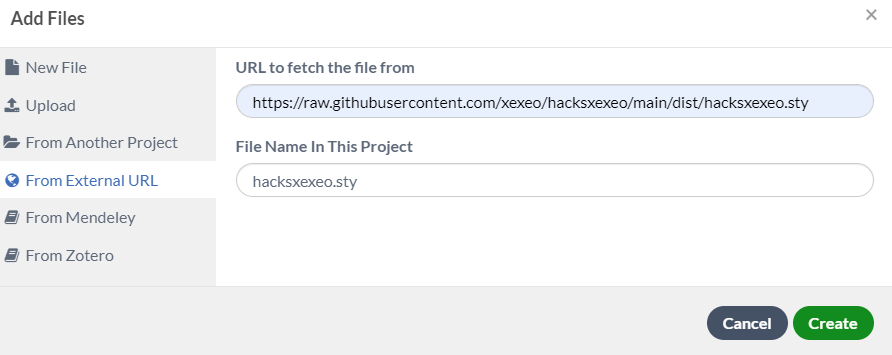
\includegraphics[width=0.7\linewidth]{../../images/overleaffileurl}
      \caption{Test Image for LoC}
      \label{fig:overleaffileurl}
  \end{figure}


  \chapter{Resultados e Discuss\~oes}
  \chapter{Conclus\~oes}

  \backmatter
  \bibliographystyle{coppe-unsrt}
  \bibliography{example}

  \appendix
  \chapter{Algumas Demonstra{\c c}\~oes}
\end{document}
%%
%%
%% End of file `example.tex'.
